\documentclass[11.5pt, paper=a4]{article}

\usepackage[utf8]{inputenc}
\usepackage[english]{babel}
\usepackage[T1]{fontenc}

\usepackage{amsmath, amssymb, amscd, amsthm, amsfonts, mathtools}
\usepackage[left=2cm, right=2cm, top=1.5cm]{geometry}

\usepackage{graphicx}
\usepackage{hyperref}
\usepackage{physics}
\usepackage{tikz}
\usepackage{url}
\usepackage[square,numbers]{natbib} \usepackage{tabularx}

\usepackage{braket}
\usepackage{thmtools}
\usepackage{float}

%%% Theorem Style
\theoremstyle{definition}
\newtheorem{theorem}{Theorem}[section]
\newtheorem{definition}[theorem]{Definition}
\newtheorem{lemma}[theorem]{Lemma}
\newtheorem{conjecture}[theorem]{Conjecture}
\newtheorem{corollary}[theorem]{Corollary}

\numberwithin{theorem}{section}

%% Autoref prefixes
\renewcommand{\sectionautorefname}{Section}
\renewcommand{\subsectionautorefname}{Section}
\renewcommand{\subsubsectionautorefname}{Section}
\renewcommand{\figureautorefname}{Figure}
\def\theoremautorefname{Theorem}
\def\lemmaautorefname{Lemma}
\def\definitionautorefname{Definition}
\def\conjectureautorefname{Conjecture}
\def\algorithmautorefname{Algorithm}

%% Writing algorithms

\usepackage{algorithm} % captioning
\usepackage{algpseudocode}

% \def\NoNumber#1{{\def\alglinenumber##1{}\State #1}\addtocounter{ALG@line}{-1}}



\title{Quantum Algorithms, Spring 2022: Lecture 3 Scribe}

\author{Alapan Chaudhuri, Zeeshan Ahmed}

\date{Jan 11, 2022}

\begin{document}

\maketitle

\section{Postulates of Quantum Mechanics}
\subsection{Hilbert Space}
Any isolated physical system is given by its state vector which is a unit vector belonging to a Hilbert Space corresponding to the system's state space.

Given Hilbert space $\mathbf{H}$ corresponding to the state space of the system, the state of the system can be represented by $\ket{\psi} \in \mathbf{H}$ such that $\bra{\psi}\ket{\psi} = 1$.

\subsection{Evolution}
Evolution of a closed quantum system is given by a unitary transformation. In its physical interpretation we have this postulate governed by the Schrodinger Equation, as stated below.
$$
i{\hslash}\frac{d\vert\psi\rangle}{dt} = H\vert\psi\rangle
$$
The above leads to $\ket{\psi(t)} = e^{-iHt}\ket{\psi(0)}$, given that the Hamiltonian itself is not dependent on time. The Hamiltonian is a self-adjoint operator and has a spectral decomposition, $H = \sum E\vert E\rangle\langle E\vert$. Furthermore, here $e^{-iHt}$ serves as the unitary transformation over time $t$ on $\ket{\psi(0)}$.\newline

It is worth noting that both Hermitian and unitary matrices have their associated spectral decomposition. In case of Hermitian matrices, the eigenvalues are real whereas for unitary matrices the absolute value of each eigenvalue is $1$. Moreover, eigenvectors of a unitary matrix are orthogonal if they have different eigenvalues.

\subsubsection{Trace preservation}
To ensure that the evolution maintains the state vector to be a unit vector, the operators preserve trace. Unitary operations satisfy this property:
\begin{align*}
    \ket{\psi_1'} = U \ket{\psi_1} \\
    \ket{\psi_2'} = U \ket{\psi_2} \\
    \bra{\psi_1'}\ket{\psi_2'} = \bra{\psi_1}U^\dag U \ket{\psi_2} \\
    \bra{\psi_1'}\ket{\psi_2'} = \bra{\psi_1} I \ket{\psi_2} \\
    \bra{\psi_1'}\ket{\psi_2'} = \bra{\psi_1} \ket{\psi_2} \\
\end{align*}
Trace preserving operators also convert a mutually orthonormal set of vectors to another mutually orthonormal set of vectors.

\subsection{Composition}
The state space of a composite physical system is the tensor product of the state spaces of the component systems.
$$
\vert\psi\rangle = \vert\psi_1\rangle\otimes...\otimes\vert\psi_n\rangle
$$
There are states in this composite physical system that can not be factorized into states of the individual systems, these states are called \textbf{entangled} states. An example in space $\mathbb{C}^4$ would be:
\begin{equation*}
    \frac{\ket{00} + \ket{11}}{\sqrt{2}}
\end{equation*}
The above state is also referred to as the a bell state.

\subsection{Measurement}
Quantum measurements are described by a collection $\{M_m\}$ of measurement operators acting on the state space of the system. \newline

We would be mostly dealing with projective measurements which are defined using observables like $M = \sum \lambda_m \ket{m}\bra{m}$. Here, $\{\lambda_m\}$ is the set of outcomes and $\{M_m = \ket{m}\bra{m}\}$ is the collection of measurement operators, as mentioned before.\newline

Probability that upon measurement the outcome is $m$ is given my $p(m) = \langle\psi\vert M_m^\dagger M_m\vert\psi\rangle = \braket{\psi}{m}\braket{m}{\psi} = \vert\braket{m}{\psi}\vert^2$ and the state of the system collapses.
$$
\vert\psi\rangle \xrightarrow{\text{on measuring}} \frac{M_m\vert\psi\rangle}{\sqrt{p(m)}} = \ket{m}
$$

Furthermore, $\sum_m p(m) = \bra{\psi} (\sum \ket{m}\bra{m}) \ket{\psi} = \braket{\psi}{\psi} = \vert \ket{\phi} \vert^2 = 1$.

\subsection{Qubit Measurement}
Consider $\ket{\psi} = a \ket{0} + b \ket{1}$. Here, let our measurement operators be $M_0 = \ket{0}\bra{0}$ and $M_1 = \ket{1}\bra{1}$. Then, we have corresponding probabilities as follows.

$$p(0) = \vert \braket{0}{\psi} \vert^2 = \vert a \vert^2$$
$$p(1) = \vert \braket{1}{\psi} \vert^2 = \vert b \vert^2$$
$$\vert a\vert^2 + \vert b \vert^2 = 1$$

\section{Circuit Model of Quantum Computation}
\begin{enumerate}
    \item \textbf{Initialization}: $\ket{\psi_0} = \ket{0}^{\otimes n}$
    \item \textbf{Evolution}: $\ket{\psi_t} = U_tU_{t-1}\ldots U_1\ket{\psi_0}$
    \item \textbf{Measurement}: Typically we perform measurements in a computational basis. $$p_t(f) = \vert \braket{f}{\psi} \vert$$
\end{enumerate}

\section{Classical Circuit}

In classical computers, we often perform irreversible computations involving gates such as AND and OR. Now, according to Landauer's principle, information loss leads to heat dissipation which means that irreversible computation by leads to heat dissipation.\newline
On the other hand, reversible computing doesn't lead to any heat dissipation. Quantum computing is inherently reversible since every computation is represented by unitary gates which are reversible by definition.

\subsection{Universal Gates}
All possible boolean functions can be constructed using circuits made with a single gate. These gates are called universal gates. An example in the classical circuits domain would be NAND gate.

Given that quantum circuits must be reversible, the individual components, i.e. the gates must be reversible in nature too. Which leads us to a proven universal gate in quantum circuits.


\subsection{Fredkin Gate}
Fredkin Gate, also known as the controlled SWAP gate, is an example of a reversible quantum gate (unitary gate) which serves as an universal gate as well.
\begin{figure}[H]
    \centering
    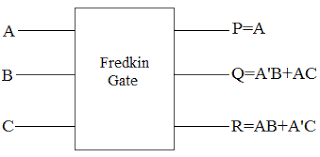
\includegraphics[width=70mm]{images/fredkin_basic.png}
    % \caption{Caption}
    \label{fig:my_label}
\end{figure}

We can show that this gate is universal in the classical domain by constructing AND and OR using the Fredkin Gate.

\begin{figure}[H]
    \centering
    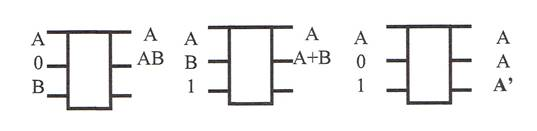
\includegraphics[]{images/fredkin.jpg}
    % \caption{Caption}
    \label{fig:my_label}
\end{figure}

\section*{Exercises}
\subsection{Entangled States}
To show that the bell state is an entangled state and can't be factorized into individual 2 qubit system states.
\begin{equation*}
    \ket{\psi} = \frac{\ket{00} + \ket{11}}{\sqrt{2}}
\end{equation*}
\subsubsection{Solution}
A product state which is not an entangled state represented in computational basis without normalization can be generalized as:
\begin{align*}
    \ket{\psi} = (a_0 \ket{0} + a_1 \ket{1})(b_0\ket{0} + b_1\ket{1}) \\
    \ket{\psi} = a_0 b_0\ket{00} + a_0 b_1\ket{01} + a_0 b_1\ket{10} + a_1 b_1\ket{11}
\end{align*}
Matching the amplitudes with the amplitudes of the bell state we get:
\begin{align*}
    a_0b_0 = 1 \\ a_0b_1 = 0 \\ a_1b_0 = 0 \\ a_1b_1 = 1
    a_0 = 0 \text{or} b_1 = 0
\end{align*}
This leads to a contradiction since $a_0b_0 = 1$ and $a_1b_1 = 1$. Hence proved.

\nocite{*}
\bibliographystyle{plainnat}
\bibliography{references}

\end{document}
